\documentclass[12pt,a4paper]{article}
\usepackage[utf8]{inputenc}
\usepackage{graphicx}
\usepackage{geometry}
\usepackage{enumitem}
\usepackage{titlesec}
\usepackage{hyperref}

\geometry{margin=2.5cm}

\title{Course Income Analysis}
\date{}

\begin{document}

\maketitle

\section*{1. Monthly Income Trend}

The total monthly income shows a generally upward trajectory with some fluctuations (see Figure~\ref{fig:monthly-income}). Income reached its lowest point in March 2022, then peaked in July 2022 with over 2.06 billion IRR. From August onward, income remained relatively high and stable, indicating a strong second half of the year in terms of revenue.

\begin{figure}[h!]
    \centering
    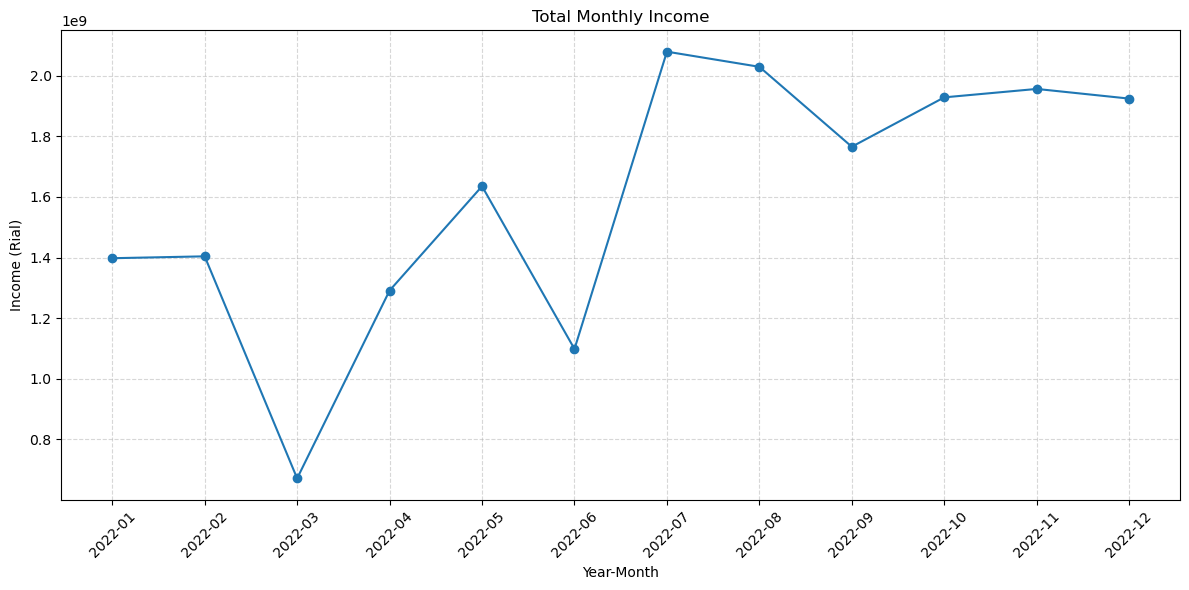
\includegraphics[width=0.90\textwidth]{Total Monthly Income.png}
    \caption{Total Monthly Income}
    \label{fig:monthly-income}
\end{figure}

\section*{2. Income by Course Type}

As illustrated in Figure~\ref{fig:income-by-course-type}, Barista courses dominate revenue, generating more than 8.3 billion IRR, significantly higher than any other course. The next highest contributors are Pizza (3.28B IRR), Sausage (1.71B IRR), and Burger (1.66B IRR).

Traditional and Kabab courses generated the least income, suggesting lower popularity or pricing.

\begin{figure}[h!]
    \centering
    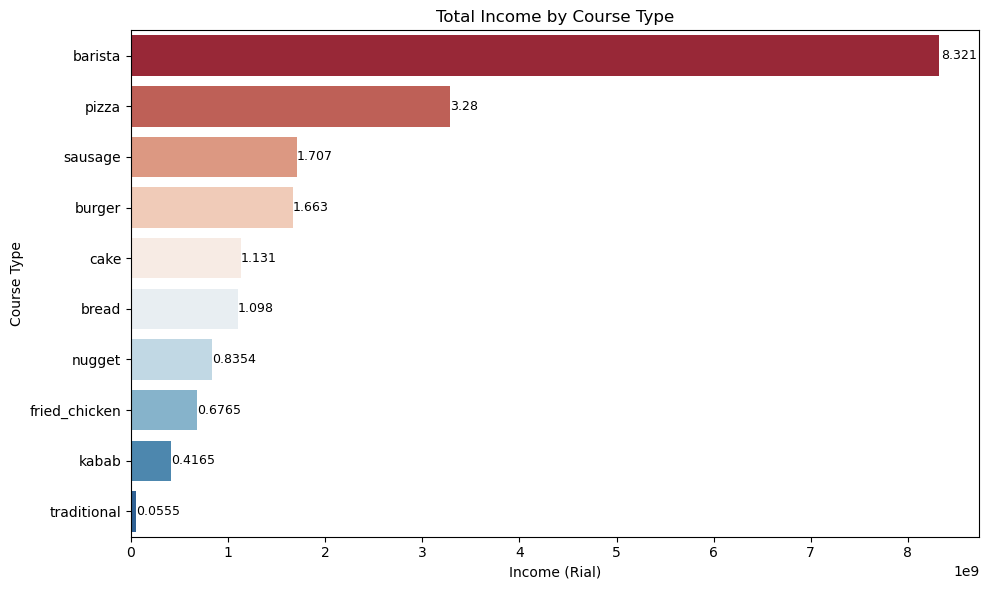
\includegraphics[width=0.92\textwidth]{Total Income by Course Type.png}
    \caption{Total Income by Course Type}
    \label{fig:income-by-course-type}
\end{figure}

\section*{3. Seasonal Income Distribution}

As shown in Figure~\ref{fig:income-by-season}, the highest income was recorded in Summer (5.88B IRR), followed closely by Autumn (5.81B IRR). Spring (4.02B IRR) and Winter (3.47B IRR) had lower contributions. The seasonal pattern aligns with higher student participation in Summer and Autumn, suggesting favourable conditions for course offerings during these times.

\begin{figure}[h!]
    \centering
    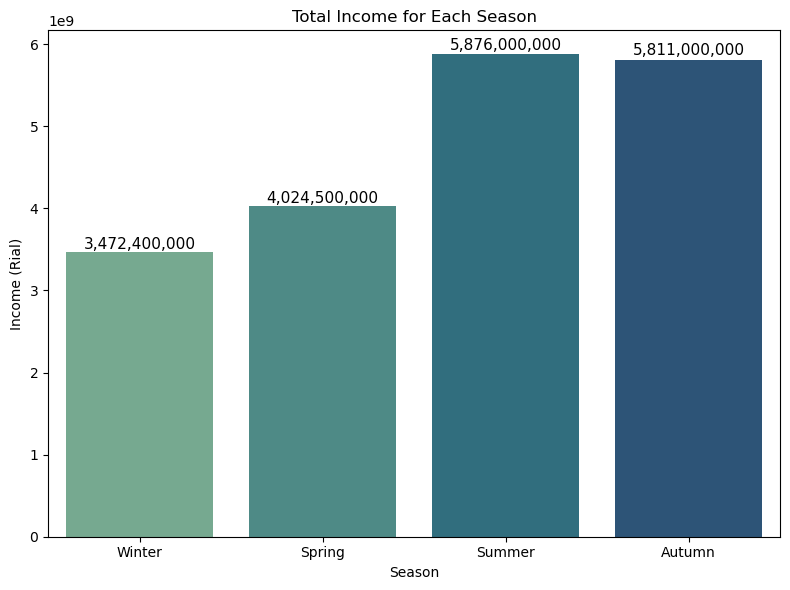
\includegraphics[width=0.65\textwidth]{Total Income for Each Season.png}
    \caption{Total Income for Each Season}
    \label{fig:income-by-season}
\end{figure}

\section*{Summary}

\begin{itemize}
    \item Barista courses are the top revenue generators by a large margin.
    \item Income has a generally increasing trend throughout the year, with the strongest revenue in the second half.
    \item Summer and Autumn are peak revenue seasons, consistent with student enrollment patterns.
    \item Less popular courses contribute marginally to overall income, indicating potential areas for growth or reconsideration.
\end{itemize}

\end{document}